\chapter{THE OPTIMIZATION METHODS}
\section*{Introduction:}
Sometimes, there are more then one way to solve a problem. We need to learn how to compare the performance of different algorithms and choose the best one to solve a particular problem. When analyzing an algorithm, we mostly consider a computational complexity which is divided into: Time complexity and Space complexity.
Heuristic and metaheuristic techniques are used for solving computational hard optimization problem. Local search is a heuristic technique while Ant Colony Optimization (ACO), inspired by the ants' foraging behavior, is one of the most recent metaheuristic technique. These technique are used for solving optimization problems.
\section{Optimization Methods:}
Following the complexity of the problem, it may be solved by an exact method or an approximate method (Figure2). Exact methods obtain optimal solution and guarantee ether optimality. For NP-complete problems, exact algorithms are non polynomialtime algorithms (unless P=NP).
Approximate (or heuristic) methods generate  high quality solutions in reasonable time for practical use, but there is not guarantee of finding a global optimum solution.
\section{Classification of optimization methods:}
\begin{figure}[H]
	\begin{center}
		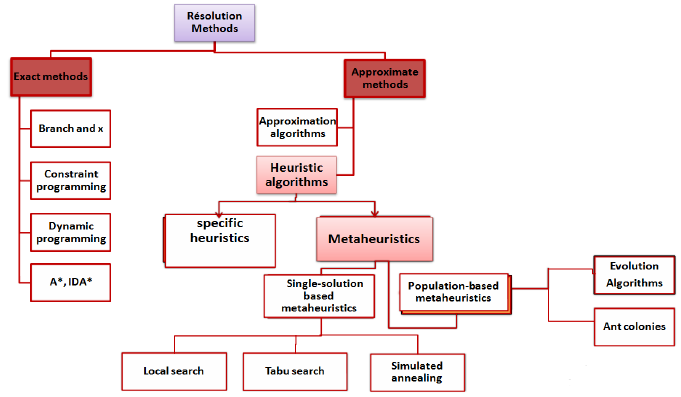
\includegraphics[scale=0.8]				{Figure2.png}
		\caption{Classical Optimization 		Methods}
	\end{center}
\end{figure}
\newpage
\subsection{Exact Methods:}
Exact methods seek to find the optimal solution with certainly by explicitly or implicitly examining the entire search space. They have advantage of guaranteeing the optimal solution, however, the computational time necessary for reaching this solution become very excessive depending on the size of the problem (combinatorial explosion)and the number of objectives to optimize. What limits the use of this type of methods for small size problems. These generic methods are: Branch \& bound, Branch \& cut and Branch \& price, other methods are less general, such as: linear programming in integer, the algorithm of A *. Other methods are specific to a given problem like Johnson's algorithm for scheduling.\\
In class of exact methods we can find the following classical algorithms:\\
Dynamic programming, branch and X family of algorithms (branch and bound, branch and cut, branch and price) developed in operations research community, constraint algorithms, and $A^{*}, IDA^{*}$ iterative deepening algorithms) developed in artificial intelligence community.\\
Those enumerative methods may be viewed as tree research algorithms.The search is carried out over the whole interesting search space, and the problem is solved by subdividing it into simple problems.
\\subsubsection{Dynamic Programming:}
is based recursive division of a problem into simpler subproblems. This procedure is based into  Bellman's principle that says that " The subpolicy of an optimal policy is itself optimal".\\
This stagewise optimization method is a result of a sequence of partial decisions. The procedure avoids the total enumeration of the search space by pruning partial decisions sequence that cannot lead to the optimal solution.
\subsubsection{The branch and bound algorithms and $A^{*}$:}
are based on an implicit enumeration of all solutions of the considered optimization problem. The search space is explored by dynamically building a tree whose root node represents the problem being solved and its whole associated search space.\\
The leaf nodes are the potential solutions and the internal nodes are subproblems of the total solution space. The pruning of the search tree is based on a bounding function that prunes subtrees that do not contain any optimal solution.
\subsubsection{Constraint Programming:}
is a language built around concepts of tree search and logical implications. Optimization problems in constraint programming are modeled by means of a set of variables linked by a set of constraints. The variables take their values on a finite domain of integers. The constraints may have mathematical or symbolic forms.\\
Exact methods can be applied to small instances of difficult problems. Table 2 shows for some popular NP hard optimization problems the order of magnitude of the maximal size of instances that state-of-the-art exact methods can solve to optimality.
\begin{figure}[H]
	\begin{center}
		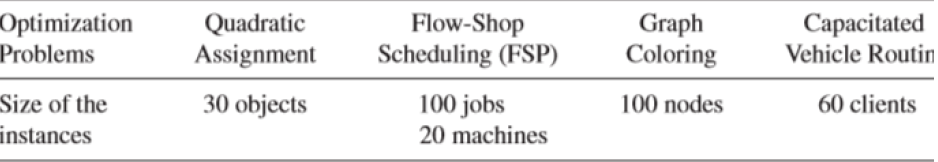
\includegraphics[scale=0.7]	{table2.png}
		\caption{TABLE 2 Order of Magnitude of the Maximal Size of Instances that State-of-the-Art Exact Methods can Solve to Optimality}
	\end{center}
\end{figure}
Some of the exact algorithms used are implemented on large networks of workstations (grid computing platforms) composed of more than 2000 processors with more than 2 months of computing time [546]! The size of the instance is not the unique indicator that describes the difficulty of a problem, but also its structure. For a given problem, some small instances cannot be solved by an exact algorithm while some large instances may be solved exactly by the same algorithm.
\subsection{Approximate	methods:}
In the class of approximate methods, two subclasses of algorithms may be distinguished: approximation algorithms and heuristic algorithms.Unlike heuristics ,which usually find reasonably “good” solutions in a reasonable time, approximation algorithms provide provable solution quality and provable run-time bounds. Heuristics find “good” solutions on large-size problem instances. They allow to obtain acceptable performance at acceptable costs in a wide range of problems. In general, heuristics do not have an approximation guarantee on the obtained solutions. They may be classified into two families: specific heuristics and metaheuristics. Specific heuristics are tailored and designed to solve a specific problem and/or instance. Metaheuristics are general purpose algorithms that can be applied to solve almost any optimization problem. They maybe viewed as upper level general methodologies that can be used as a guiding strategy in designing underlying heuristics to solve specific optimization problems.
\subsubsection{Definition $\varrho$-Approximation algorithms:}
An algorithm has an approximation factor $\varrho$if its time complexity is polynomial and for any input instance it produces a solution a such that\\
\begin{subequations}
\renewcommand{\theequation}{\arabic{parentequation}--\arabic{equation}}
\begin{align}
    a \le \epsilon * \text{s} \vspace{0.5cm} & \text{ if }\epsilon > 1\\
    \epsilon * s \le \text{a} \vspace{0.5cm} & \text{ if }\epsilon < 1
\end{align}
\end{subequations}
